\section{Potencial eléctrico}
\label{sec:potencial}

Así como el concepto de trabajo y energía hizo posible resolver con facilidad algunos problemas de mecánica, el empleo de las ideas de energía también hace más fácil la solución de una variedad de problemas de electricidad.

Cuando una partícula con carga se mueve por un campo eléctrico, el campo ejerce una fuerza que efectúa trabajo sobre la partícula. Este trabajo siempre se puede expresar en términos de la energía potencial eléctrica. Así como la energía potencial gravitatoria depende de la altura de una masa sobre la superficie terrestre, la energía potencial eléctrica depende de la posición que ocupa la partícula con carga en el campo eléctrico. Describiremos la energía potencial eléctrica utilizando un concepto llamado \emph{potencial eléctrico} o simplemente potencial.

\begin{tcolorbox}[interesting_data]
  A modo de recordatorio, el trabajo \(W_{ab}\) realizado por una fuerza \(\vec{F}\) sobre una partícula para desplazarla desde el punto \(a\) al punto \(b\) se define como 
  \[
    W_{ab}=\int_a^b \vec{F}\cdot d\vec{s}
  \]
  Donde la fuerza \(\vec{F}(s)\) es una función con respecto a la posición, y por lo tanto depende del desplazamiento \(d\vec{s}\).

  Por otro lado, si la fuerza \(\vec{F}\) resultaba ser conservativa, entonces el trabajo se podía expresar en términos de una energía potencial \(U\). Para que la partícula experimente una fuerza, debía existir un cambio en su velocidad (es decir, una aceleración). Si este cambio era debido a la fuerza peso, resultaba ser que había un cambio en su energía potencial que podía expresarse como \(\Delta U=U_b-U_a\), y el trabajo resulta
  \[
    W_{ab}=U_a - U_b = -(U_b - U_a) = -\Delta U
  \]
  De esta última expresión se puede concluir que si el trabajo resulta positivo entonces la energía potencial en \(a\) es mayor que en \(b\), y significa que el campo realizó un trabajo sobre la partícula, es decir, \(\Delta U\) es negativo porque se perdió energía potencial y se ganó energía cinética. Ocurre lo contrario si el trabajo resulta negativo.

  Por último, para terminar la revisión, el teorema del trabajo y la energía establece que el \emph{cambio} en la energía cinética \(\Delta K\) durante cualquier desplazamiento es igual al trabajo total realizado sobre la partícula. Si el único trabajo efectuado sobre la partícula lo realizan fuerzas conservativas, entonces 
  \[
    \Delta K = - \Delta U \qquad \Rightarrow \qquad K_a + U_a = K_b + U_b
  \]
  Es decir, la energía total (cinética más potencial) se conserva.
\end{tcolorbox}

Volviendo con electrostática, cuando se coloca una carga de prueba \(q_0\) en un campo eléctrico \(\vec{E}\), la carga experimenta una fuerza eléctrica \(\vec{F_e}=q_0\vec{E}\). Esta fuerza es conservativa, lo que significa que el trabajo realizado por la fuerza al mover la carga entre dos puntos \(A\) y \(B\) no depende de la trayectoria seguida, sino solo de los puntos inicial y final.

El trabajo realizado por la fuerza al mover la carga \(q_0\) desde el punto \(A\) hasta el punto \(B\) se define como
\begin{equation*}
  W_{AB} = \int_A^B \vec{F_e} \cdot d\vec{s} = \int_A^B q_0\vec{E} \cdot d\vec{s}
\end{equation*}
Y como la fuerza eléctrica es conservativa, podemos expresarla en términos de la energía potencial eléctrica \(U\),
\begin{equation*}
  W_{AB} = U_A - U_B = -\Delta U = \int_A^B \underbrace{q_0\vec{E}}_{\vec{F}_e} \cdot d\vec{s}
\end{equation*}
\begin{tcolorbox}[myconclusion]
  Recuerde que la fuerza es una función, por tanto es lo que se busca integrar.
\end{tcolorbox}
Entonces, para el trabajo realizado por una fuerza eléctrica, lo que importa es cómo varía la fuerza a lo largo del desplazamiento. Como la fuerza eléctrica es una fuerza conservativa, el trabajo no depende de la trayectoria seguida por la carga de prueba \(q_0\), sino únicamente de la diferencia de energía potencial entre las posiciones inicial y final del trayecto.

La energía potencial eléctrica \(U\) del sistema depende de la configuración espacial de las cargas. Para deducir su valor absoluto, es necesario establecer un punto de referencia donde la energía potencial sea cero. En el caso de un campo generado por una carga puntual \(q\), es conveniente establecer este nivel cero en el infinito, donde las cargas están tan alejadas que no interactúan. 

\begin{marginfigure}
  \centering
  \caption{Gráfica de la energía potencial \(U\) de dos cargas puntuales contra su separación \(r\).}
  \label{fig_funcion_energia_potencial}
  \begin{tikzpicture}[>=stealth]
  \begin{axis}[
      axis lines = middle, 
      xlabel={$r$},
      ylabel={$U$},
      ymin=-0.5, ymax=6.5,
      xmin=-0.5, xmax=6.5,
      xtick=\empty,
      ytick=\empty,
      domain=0.17:5.5, 
      samples=100,
      grid=none,
      width=\marginparwidth,
      height=\marginparwidth,
      axis line style={gray}
    ]
    \addplot[teal, very thick] {1/x};
  \end{axis}
  \shade[ball color=orange] (1,2) circle (.15) node[above=1mm] {\scriptsize$q$};
  \shade[ball color=orange] (2,2) circle (.15) node[above=1mm] {\scriptsize$q_0$};
  \draw[thin] (1,1.8) -- (1,1.6);
  \draw[thin] (2,1.8) -- (2,1.6);
  \draw[thin,<->] (1,1.7) -- node[below] {$r$} (2,1.7);
  \shade[ball color=blue!40] (1,2.7) circle (.15) node[above=1mm] {\scriptsize$q$};
  \shade[ball color=blue!40] (2,2.7) circle (.15) node[above=1mm] {\scriptsize$q_0$};
\end{tikzpicture}
\vspace{1cm}
\begin{tikzpicture}[>=stealth]
  \begin{axis}[
      axis lines = middle, 
      xlabel={$r$},
      ymin=-6.5, ymax=0.5,
      xmin=-0.5, xmax=6.5,
      xtick=\empty,
      ytick=\empty,
      domain=0.17:5.5, 
      samples=100,
      grid=none,
      width=\marginparwidth,
      height=\marginparwidth,
      axis line style={gray}
    ]
    \addplot[teal, very thick] {-1/x};
  \end{axis}
  \shade[ball color=blue!40] (1,1) circle (.15) node[above=1mm] {\scriptsize$q$};
  \shade[ball color=orange] (2,1) circle (.15) node[above=1mm] {\scriptsize$q_0$};
  \draw[thin] (1,0.8) -- (1,0.6);
  \draw[thin] (2,0.8) -- (2,0.6);
  \draw[thin,<->] (1,0.7) -- node[below] {$r$} (2,0.7);
  \shade[ball color=orange] (1,1.7) circle (.15) node[above=1mm] {\scriptsize$q$};
  \shade[ball color=blue!40] (2,1.7) circle (.15) node[above=1mm] {\scriptsize$q_0$};
  \node (cartel) [
    text width=3cm,
    align=left,
    fill=yellow!40!black!14,
    draw=yellow!40!black!46,
    thick,
    rounded corners=2pt,
    inner sep=2mm
    ]
    at (1.35,-2) {\footnotesize{Cuando las cargas son iguales, el potencial es mayor si la distancia es menor. Lo contrario ocurre cuando son distintas.}};
\end{tikzpicture}

\end{marginfigure}
De esta forma, la energía potencial \(U\) del sistema formado por una carga fuente \(q\) y una carga de prueba \(q_0\) separadas por una distancia \(r\), equivale al trabajo realizado por un agente externo para traer la carga de prueba desde el infinito hasta dicha distancia \(r\) sin aceleración:
\[
  U = k_e\frac{q q_0}{r}~ [\unit{\joule}]
\]
donde \(r\) es la distancia entre la carga de prueba \(q_0\) y la carga fuente \(q\).

Como se puede intuir, este punto de referencia de energía potencial cero depende de la configuración de cargas y del campo; si bien suele fijarse en el infinito para cargas puntuales (como muestra la figura \ref{fig_funcion_energia_potencial}), en otros sistemas prácticos puede convenir fijarlo en otro lugar, como en la superficie de un conductor o en la ``tierra''.

\subsection{Definición de potencial eléctrico}

\begin{definition}[Potencial Eléctrico]\label{def_potencial}
Para una posición conocida de la carga de prueba en el campo, el sistema carga-campo tiene una energía potencial \(U\) relativa a la configuración del sistema definida como \(U=0\). Al dividir la energía potencial entre la carga de prueba \(q_0\), obtenemos el \emph{potencial eléctrico} \(V\) en un punto \(P\) del campo eléctrico:
\begin{equation}
  V = \frac{U}{q_0} ~ [\unit{\joule\per\coulomb}]
  \label{eq:potential}
\end{equation}
\end{definition}

El potencial eléctrico es una magnitud escalar que se mide en \unit{\volt} (voltios)\footnote{Observe el importante detalle tipográfico, el potencial eléctrico se denota con una \(V\) mayúscula itálica, mientras que la unidad voltio se denota con una \unit{\volt} mayúscula regular.} y se define como la energía potencial por unidad de carga.
% En versiones futuras, se podría usar \(\mathcal{V}\) en vez de V, para evitar confusión.

Teniendo en cuenta la definición \ref{def_potencial} de potencial y la ecuación \eqref{eq:potential}, se define la diferencia de potencial \(\Delta V = V_B - V_A\) entre dos puntos \(A\) y \(B\) en un campo eléctrico. Esto representa el cambio de energía potencial por unidad de carga al mover una carga de prueba \(q_0\) entre esos dos puntos
\begin{equation}
  \Delta V = \frac{\Delta U}{q_0} = -\int_A^B \vec{E} \cdot d\vec{s}
  \label{eq:potential_difference}
\end{equation}

Por la ecuación \eqref{eq:potential_difference}, el trabajo realizado por un agente externo al desplazar una carga \(q\) a través de un campo eléctrico con una velocidad constante es:
\[
  W=q\Delta V
\]

Es muy importante que el desplazamiento de la carga \(q\) sea a velocidad constante, ya que si no lo es, el trabajo realizado por el agente externo no será igual al trabajo realizado por la fuerza eléctrica. 

\begin{tcolorbox}[myconclusion]
  Cuando se habla de un agente externo y desplazamiento a velocidad constante (o sin aceleración) es importante entender que se busca que \(\Delta K = 0\). De esta forma el trabajo total que es el cambio en la energía cinética más el cambio en la energía potencial resultará 
  \[
    W = \Delta U + \cancel{\Delta K}
  \]
\end{tcolorbox}
\begin{figure}[!ht]
  \centering
  \begin{subfigure}[b]{0.45\textwidth}
    \centering
    \begin{tikzpicture}[>=stealth]
      \coordinate (A) at (0,1);
      \coordinate (B) at (0,-1);
      \begin{scope}[very thick,decoration={
          markings,
          mark=at position 0.6 with {\arrow{>}}
        }] 
        \foreach \x in {-1,-.5,...,1} {
          \draw[orange, thick,postaction=decorate] (\x,1.5) -- (\x,-1.5);
        }
      \end{scope}
      \shade[ball color=orange, opacity=0.3, text opacity=1] (A) circle (.2) node[left=1mm] {\scriptsize{A}};
      \shade[ball color=orange] (B) circle (.2) node[left=1mm] {\scriptsize{B}};
      \draw[thin] ($(A)+(0.4,0)$) -- ($(A)+(0.9,0)$);
      \draw[thin] ($(B)+(0.4,0)$) -- ($(B)+(0.9,0)$);
      \draw[thin,<->] ($(A)+(.75,0)$) -- node[fill=white,inner sep=1pt] {$d$} ($(B)+(.75,0)$);
      \node at (-1.3,-1) {$\vec{E}$};

      \node (cartel) [
        font=\footnotesize,
        text width=4.5cm,
        align=left,
        fill=yellow!40!black!14,
        draw=yellow!40!black!46,
        thick,
        rounded corners=2pt,
        inner sep=2mm
        ]
        at ($(A)+(0,1.7)$) {Cuando una carga de prueba positiva se mueve del punto A al punto B, la energía potencial eléctrica del sistema carga-campo disminuye.};
    \end{tikzpicture}
  \end{subfigure}
  \begin{subfigure}[b]{0.45\textwidth}
    \centering
    \begin{tikzpicture}[>=stealth]
      \coordinate (A) at (0,1);
      \coordinate (B) at (0,-1);
      \begin{scope}[very thick,decoration={
          markings,
          mark=at position 0.6 with {\arrow{>}}
        }] 
        \foreach \x in {-1,-.5,...,1} {
          \draw[blue!50, thick,postaction=decorate] (\x,1.5) -- (\x,-1.5);
        }
      \end{scope}
      \shade[ball color=blue!50, opacity=0.3, text opacity=1] (A) circle (.2) node[left=1mm] {\scriptsize{A}};
      \shade[ball color=blue!50] (B) circle (.2) node[left=1mm] {\scriptsize{B}};
      \draw[thin] ($(A)+(0.4,0)$) -- ($(A)+(0.9,0)$);
      \draw[thin] ($(B)+(0.4,0)$) -- ($(B)+(0.9,0)$);
      \draw[thin,<->] ($(A)+(.75,0)$) -- node[fill=white,inner sep=1pt] {$d$} ($(B)+(.75,0)$);
      \node at (-1.3,-1) {$\vec{g}$};

      \node (cartel) [
        font=\footnotesize,
        text width=4.5cm,
        align=left,
        fill=yellow!40!black!14,
        draw=yellow!40!black!46,
        thick,
        rounded corners=2pt,
        inner sep=2mm
        ]
        at ($(A)+(0,1.7)$) {Cuando un objeto con masa se mueve del punto A al punto B, la energía potencial gravitacional del sistema objeto-campo disminuye.};
    \end{tikzpicture}
  \end{subfigure}
  \caption{Comparación de la energía potencial eléctrica y gravitatoria.}
  \label{fig_potential_uniform}
\end{figure}


Nótese que el concepto de potencial eléctrico se concibe de forma similar al de campo eléctrico. Se usa una carga de prueba positiva \(q\) haciendo que sólo dependa de la carga fuente \(Q\) que genera el campo eléctrico. 

\subsection{Diferencia de potencial en un campo eléctrico uniforme}

La ecuación \eqref{eq:potential_difference} es válida en todos los campos eléctricos, sean uniformes o no, es decir, es la fórmula general para la obtención de la diferencia de potencial. Sin embargo, en un campo eléctrico uniforme, la magnitud del campo \(\vec{E}\) es constante y la dirección de \(\vec{E}\) es la misma en todos los puntos del campo, de modo tal que se pueden simplificar los cálculos. En este caso, la diferencia de potencial entre dos puntos \(A\) y \(B\) separados por una distancia \(d\) en la dirección del campo eléctrico se puede expresar como:
\begin{equation}
  \Delta V = -\int_A^B \vec{E} \cdot d\vec{s} = -E \, \int_A^B ds = \boxed{-Ed}
  \label{eq:potential_uniform}
\end{equation}
donde \(E\) es la magnitud del campo eléctrico y \(d\) es la distancia entre los puntos \(A\) y \(B\) en la dirección del campo.

El signo negativo indica que el potencial en el punto \(B\) es menor que el potencial en el punto \(A\) si la carga de prueba se mueve en la dirección del campo eléctrico. Esto significa que el trabajo realizado por la fuerza eléctrica es negativo, lo que implica que la energía potencial disminuye al mover la carga en la dirección del campo eléctrico.

\begin{tcolorbox}[mydanger]
  Atención, si la carga \(q\) es negativa, la situación se invierte. El sistema gana energía potencial al mover la carga \(q\) en la dirección del campo eléctrico, y disminuye al moverla en la dirección opuesta.    
\end{tcolorbox}

\subsection{Potencial eléctrico en un punto}

\begin{marginfigure}
  \centering
  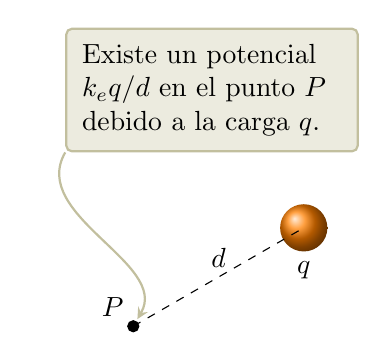
\begin{tikzpicture}[>=stealth]
    \coordinate (P) at (0,0);
    \shade[ball color=orange] (30:2.5) circle (.3) node[below=3mm] {$q$};
    \draw[dashed] (P) -- node[above] {$d$} (30:2.5);
    \filldraw (P) circle (2pt) node[above left] {$P$};
    \node (cartel) [
      text width=3.3cm,
      align=left,
      fill=yellow!40!black!14,
      draw=yellow!40!black!46,
      thick,
      rounded corners=2pt,
      inner sep=2mm
      ]
      at (1,3) {Existe un potencial $k_e q/d$ en el punto $P$ debido a la carga $q$.};
    \draw[->, thick, color=yellow!40!black!46, shorten >=3pt] 
             (cartel.south west) to[out=240, in=60] (P);
  \end{tikzpicture}
  \caption{Potencial en el punto \(P\) debido a \(q\).}
  \label{fig_potencial_en_un_punto}
\end{marginfigure}


Como se mencionó previamente, la energía potencial \(U\) es relativa a un punto que se ha definido como punto de potencial cero. Esto es importante ya que la definición de potencial eléctrico \(V\) parte del concepto de energía potencial, por cuanto, hereda estos comportamientos. Esto implica que si usted desea conocer el potencial en un punto \(P\) como muestra la figura \ref{fig_potencial_en_un_punto}, entonces primero debe saber cual es el punto de potencial cero\footnote{El potencial en un punto es simplemente un caso especial de la diferencia de potencial, donde el punto de partida (usualmente el infinito para cargas puntuales) tiene un potencial de \qty{0}{\volt}.}. De este modo, la distancia de \(P\) a dicho punto de potencial cero, dará la diferencia de potencial de \(P\) con respecto al punto de potencial cero, y consecuentemente, el potencial de \(P\). Entonces el potencial \(V\) en el punto \(P\) es el trabajo requerido para mover la carga de prueba desde el infinito hasta el punto \(P\). Aplicando la definición de potencial, el potencial en el punto \(P\) se obtiene de la siguiente manera,
\begin{align*}
    V_P &= - \lim_{a \to \infty}\int_{a}^d \vec{E} \cdot d\vec{r}\\
        &= - \lim_{a \to \infty}\int_{a}^d \frac{kq}{r^2} \cdot dr\\
        &= -kq \, \lim_{a \to \infty} \int_{a}^d \frac{1}{r^2} \cdot dr\\
        &= -kq \, \lim_{a \to \infty} \left[ -\frac{1}{r} \right]_{a}^d\\
        &= -kq \, \lim_{a \to \infty} \left[ -\frac{1}{d} + \frac{1}{a} \right]\\
        &= -kq \, \left[ -\frac{1}{d} + 0 \right] \\
    V_P &= k\frac{q}{d} = \lVert\vec{E}\rVert \, \lVert\vec{r}\rVert \cos(0)
\end{align*}
siendo \(\lVert \vec{r}\rVert\) el radiovector de módulo \(d\) que apunta a \(P\). Por ser \(\vec{E}\) y \(\vec{r}\) paralelos. Entonces el potencial eléctrico en un punto \(P\) debido a una carga puntual \(q\) es:
\begin{equation}
    \boxed{V_P = k\frac{q}{d} = E \, d}
    \label{eq:potential_point_charge}
\end{equation}
donde \(q\) es la carga fuente, \(E\) el campo generado por \(q\) y \(d\) la distancia al punto \(P\).

El potencial eléctrico debido a múltiples cargas puntuales se basa en el principio de superposición, que establece que el potencial eléctrico total en un punto es igual a la suma algebraica de los potenciales individuales producidos por cada carga.
\begin{equation}
    V_\text{total} = \sum_{i=1}^{n} V_i = k \sum_{i=1}^{n} \frac{q_i}{d_i}
\end{equation}

\subsection{Obtención de \texorpdfstring{\(\vec{E}\)}{E} a partir de \texorpdfstring{\(V\)}{V}}

El campo eléctrico \(\vec{E}\) y el potencial eléctrico \(V\) están relacionados, como se muestra en la ecuación \eqref{eq:potential_point_charge}, que se usa para encontrar \(V\) en un punto cuando se conoce \(\vec{E}\). Aunque, también podemos encontrar \(\vec{E}\) a partir de \(V\) usando la relación:
\begin{equation}
  dV = -\vec{E} \cdot d\vec{s}
  \label{eq:field_from_potential_differential}
\end{equation}
y si estamos trabajando con una única coordenada (por ejemplo, un movimiento rectilíneo) podemos escribir la ecuación \eqref{eq:field_from_potential_differential} como:
\[
  dV = -E \, ds \quad \Rightarrow \quad E = -\frac{dV}{ds}
\]

Sin embargo, en general, el potencial eléctrico es una función de las tres coordenadas espaciales. Si \(V(r)\) se da en coordenadas cartesianas, las componentes \((E_x, E_y, E_z)\) del campo eléctrico pueden ser determinadas fácilmente a partir de \(V(x, y, z)\) como derivadas parciales
\begin{equation}
  \boxed{
    \vec{E} = -\nabla V
  }
\end{equation}
donde \(\nabla\) es el operador nabla, que representa el gradiente del potencial eléctrico. Esta relación indica que el campo eléctrico es igual al negativo del gradiente del potencial eléctrico. En otras palabras, el campo eléctrico apunta en la dirección de mayor disminución del potencial eléctrico.

\begin{tcolorbox}[interesting_data,title=Recordatorio]
El operador nabla \(\nabla\) (u operador del gradiente) es una herramienta matemática usada en cálculo vectorial y análisis multivariable. Se utiliza para representar derivadas en múltiples dimensiones.

Formalmente, el operador nabla se define como:
\[
\nabla = \left( \frac{\partial}{\partial x}, \frac{\partial}{\partial y}, \frac{\partial}{\partial z} \right)
\]
Es un operador vectorial que, aplicado a diferentes tipos de funciones, da lugar a distintos conceptos. En nuestro caso solo vamos a repasar el concepto de gradiente.

Cuando se aplica el operador nabla a una función escalar \( f(x, y, z) \), produce un campo vectorial que apunta en la dirección de mayor incremento de la función. Se expresa como:
\[
\nabla f = \left( \frac{\partial f}{\partial x}, \frac{\partial f}{\partial y}, \frac{\partial f}{\partial z} \right)
\]
Este vector resultante indica la dirección en la que la función crece más rápidamente y su magnitud corresponde a la tasa de cambio máxima. En el caso de \(\vec{E}\) y \(V\), \(\vec{E}\) es el gradiente de \(V\) representa una función vectorial que apunta en la dirección de mayor aumento del potencial eléctrico.
\end{tcolorbox}
